When the observed neuron is spiking quickly, the Poisson distribution may be well approximated by a Gaussian distribution, suggesting that the Wiener filter may be optimal in this regime.  But the exponential approximation of a Poisson is also very accurate in the fast spiking regime.  To compare these two strategies, we simulated a fast spiking neuron, where the expected number of spikes per bin exceeds 10 (Fig. \ref{fig:FastSpiking}). In this scenario, both the Wiener filter and our fast filter perform approximately equally well.  Both filters infer peaks in the firing rate that are obscured by the low-pass filter properties of the calcium dynamics. Thus, it seems from this analysis that regardless of the firing rate of the observable neuron, (1) filtering the signal may provide valuable information, and (2) our fast filter performs at least as well as the Wiener filter, without requiring more computational time.


\begin{figure}[H]
\centering 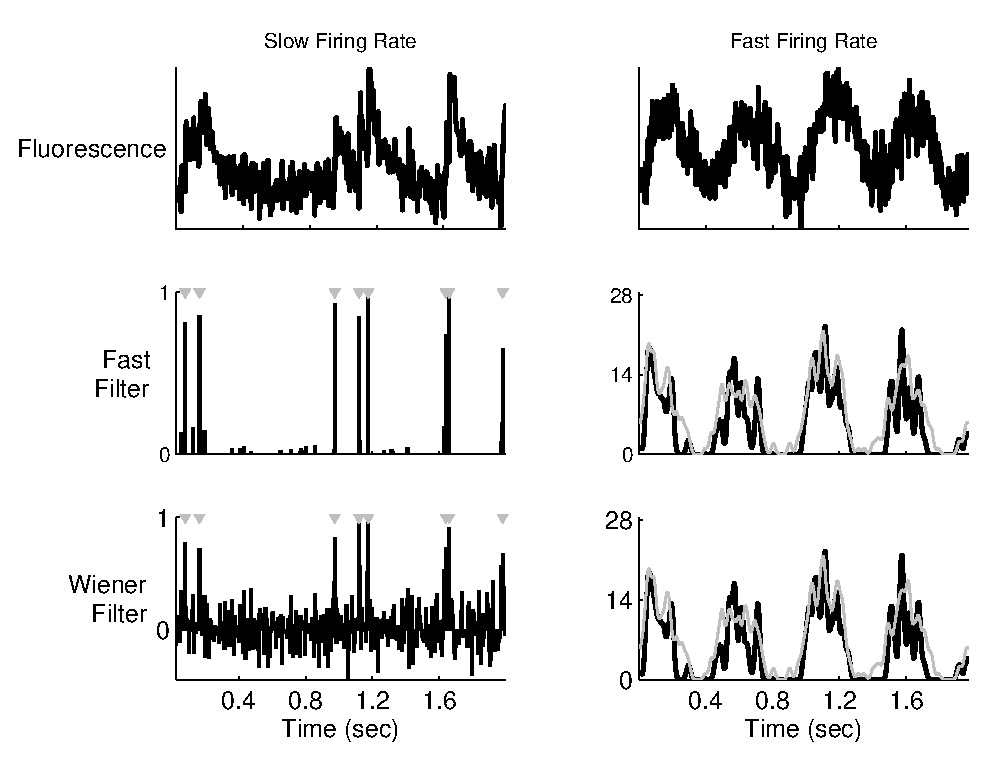
\includegraphics[width=.9\linewidth]{../figs/wiener}
\caption{A simulation demonstrating that the fast filter performs at least as well as the optimal linear filter. The left panels show that in the slow firing  regime, the fast filter --- which approximates the Poisson distribution governing spiking with an exponential distribution  --- outperforms the Wiener filter --- which approximates the Poisson distribution with a Gaussian.  The right panels show that both approximations are sufficient in the fast firing regime. Top left panel: fluorescence time series for a neuron with a slow firing rate.  Middle left panel: the fast filter's inferred spike train.  Bottom left panel: Wiener filter's inferred spike train.  Note that (i) the Wiener filter does not impose a non-negativity constraint, and (ii) the effective SNR of this filter in this example is higher than the fast filter's.  Top right panel: same as top left panel, for a neuron with a high firing rate.  Middle right panel: the fast filter's inferred spike train smoothed with a Gaussian kernel for visualization purposes (black line), and the true spike train smoothed with the same Gaussian kernel (gray line).  Bottom right panel: same as middle right panel, but with the Wiener filter. Parameters for left panels: same as above.  Parameters for right panels: same as above, except: $\sig=8$ a.u., $\lam=500$ Hz.} \label{fig:wiener}
\end{figure}

%\newpage \begin{figure}[H]
%\centering 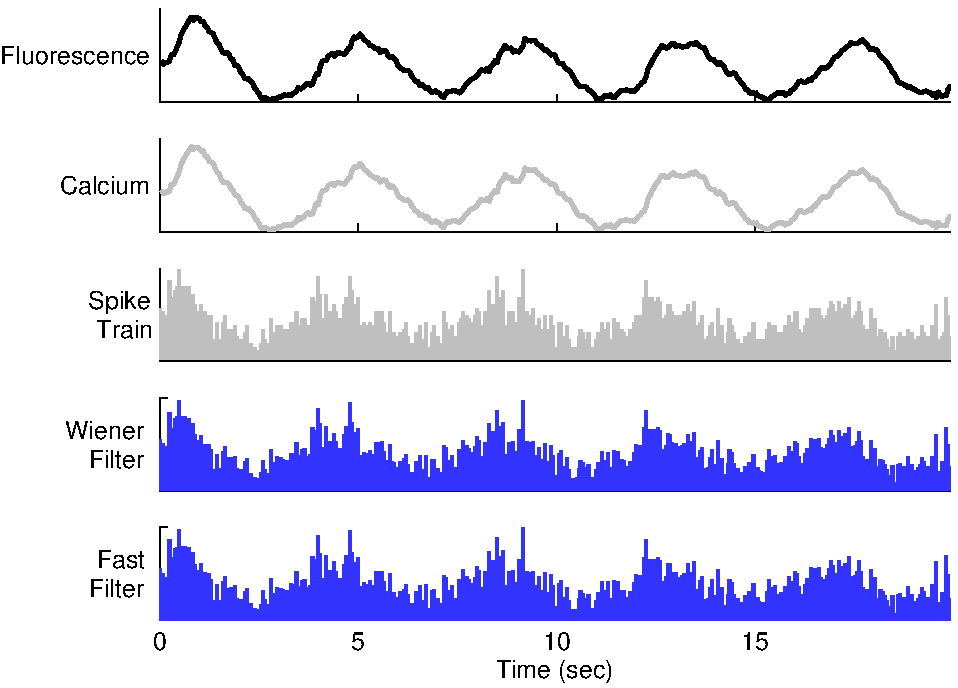
\includegraphics[width=.9\linewidth]{FastSpiking}
%\caption{Comparing the Wiener filter and our fast filter for a fast spiking neuron.  In this scenario, the two filters perform approximately equally well. Note that both recover fast fluctuations in the firing rate that are smoothed out by the calcium dynamics. Conventions as in Fig. \ref{fig:schem}.  Actual and inferred spike trains were normalized similarly, to ease comparisons. Parameters: $\gamma=0.94$, $\nu=0$, $\rho=1$, $\sig=0.3$, $\lam=100$ (modulated by a sinusoid), $\Del=0.05$ msec.} \label{fig:FastSpiking}
%\end{figure}


